\documentclass[letterpaper,11pt,oneside,reqno]{article}

%%%%%%%%%%%%%%%%%%%%%%%%%%%%%%%%%%%%%%%%%%%%%%%%%%%%%%%%%%%%

\usepackage[pdftex,backref=page,colorlinks=true,linkcolor=blue,citecolor=red]{hyperref}
\usepackage[alphabetic,nobysame]{amsrefs}

%%%%%%%%%%%%%%%%%%%%%%%%%%%%%%%%%%%%%%%%%%%%%%%%%%%%%%%%%%%%
%main packages
\usepackage{amsmath,amssymb,amsthm,amsfonts,mathtools}
\usepackage{graphicx,color}
\usepackage{upgreek}
\usepackage[mathscr]{euscript}

%equations
\allowdisplaybreaks
\numberwithin{equation}{section}

%tikz
\usepackage{tikz}
\usetikzlibrary{shapes,arrows,positioning,decorations.markings}

%conveniences
\usepackage{array}
\usepackage{adjustbox}
\usepackage{cleveref}
\usepackage{enumerate}
\usepackage{datetime}

%paper geometry
\usepackage[DIV=12]{typearea}

%%%%%%%%%%%%%%%%%%%%%%%%%%%%%%%%%%%%%%%%%%%%%%%%%%%%%%%%%%%%
%draft-specific
\synctex=1
% \usepackage{refcheck,comment}

%%%%%%%%%%%%%%%%%%%%%%%%%%%%%%%%%%%%%%%%%%%%%%%%%%%%%%%%%%%%
%this paper specific
\newcommand{\ssp}{\hspace{1pt}}

%%%%%%%%%%%%%%%%%%%%%%%%%%%%%%%%%%%%%%%%%%%%%%%%%%%%%%%%%%%%
\newtheorem{proposition}{Proposition}[section]
\newtheorem{lemma}[proposition]{Lemma}
\newtheorem{corollary}[proposition]{Corollary}
\newtheorem{theorem}[proposition]{Theorem}
%%%%%%%%%%%%%%%%%%%%%%%%%%%%%%%%%%%%%%%%%%%%%%%%%%%%%%%%%%%%
\theoremstyle{definition}
\newtheorem{definition}[proposition]{Definition}
\newtheorem{remark}[proposition]{Remark}
%%%%%%%%%%%%%%%%%%%%%%%%%%%%%%%%%%%%%%%%%%%%%%%%%%%%%%%%%%%%

\begin{document}
\title{Lectures on Random Matrices
(Spring 2025)
\\Lecture 14: Matching Random Matrices to Random Growth II}


\date{Wednesday, April 16, 2025\footnote{\href{https://lpetrov.cc/rmt25/}{\texttt{Course webpage}}
$\bullet$ \href{https://lpetrov.cc/simulations/model/random-matrices/}{\texttt{Live simulations}}
$\bullet$ \href{https://lpetrov.cc/rmt25/rmt25-notes/rmt2025-l14.tex}{\texttt{TeX Source}}
$\bullet$
Updated at \currenttime, \today}}



\author{Leonid Petrov}


\maketitle
\tableofcontents



\section{Recap}

\subsection{Main goal}

In the previous
\href{https://lpetrov.cc/rmt25/rmt25-notes/rmt2025-l13.pdf}{Lecture 13}, we began establishing a remarkable correspondence between two a~priori different objects:

\begin{itemize}
\item The \emph{spiked Wishart ensemble}: an $n\times n$ Hermitian random-matrix process $\{M(t)\}_{t\ge0}$ whose entries come from columns of independent Gaussian random vectors of suitably chosen covariance.
\item An \emph{inhomogeneous last-passage percolation (LPP)} model: an array $\{W_{i,j}\}$ of exponential random weights on a portion of the two-dimensional lattice, whose last-passage times $L(t,n)$ match the largest eigenvalues of $M(t)$, jointly for all $t\in \mathbb{Z}_{\ge0}$.
\end{itemize}

This equivalence, originally due to
\cite{dieker2008largest} (following
\cite{defosseux2010orbit}, \cite{forrester2006jacobians};
see also
\cite{Baryshnikov_GUE2001},
\cite{johansson2000shape} for earlier results of this kind),
can be fully understood by passing to a
\emph{discrete} version of LPP with geometric site-weights
and then applying the \emph{Robinson--Schensted--Knuth}
(RSK) correspondence.

\subsection{Spiked Wishart ensembles and the largest eigenvalue process}

We defined the \emph{generalized} (or spiked) Wishart matrix $M(t)$ of size $n\times n$ by setting
\[
M(t)\;=\;\sum_{m=1}^t A^{(m)}\bigl(A^{(m)}\bigr)^*
\]
where $\{A^{(m)}\}_{m=1}^\infty$ are i.i.d.\ complex Gaussian column vectors of length $n$, with
\[
\mathrm{Var}\bigl(A^{(m)}_i\bigr)
\;=\;
\frac{1}{\pi_i + \hat\pi_m}\,.
\]
Here, $\pi=(\pi_1,\dots,\pi_n)$ and $\hat\pi=(\hat\pi_1,\hat\pi_2,\dots)$ are positive and nonnegative parameters, respectively.  Writing $\lambda_1(t)\ge\cdots\ge\lambda_n(t)\ge0$ for the eigenvalues of $M(t)$, we then saw:

\begin{enumerate}
\item The vectors $\lambda(t)=\bigl(\lambda_1(t),\dots,\lambda_n(t)\bigr)$ form a Markov chain in the \emph{Weyl chamber} $\mathbb{W}^n = \{x_1\ge\cdots\ge x_n\ge0\}$.
\item There is an \emph{interlacing} property: each update $M(t-1)\mapsto M(t)$ via the rank-one matrix $A^{(t)}\bigl(A^{(t)}\bigr)^*$ forces $\lambda(t)$ to interlace with $\lambda(t-1)$:
\[
\lambda_1(t)\;\ge\;\lambda_1(t-1)\;\ge\;\lambda_2(t)\;\ge\;\cdots\;\ge\;\lambda_n(t-1)\;\ge\;\lambda_n(t).
\]
\end{enumerate}

In \href{https://lpetrov.cc/rmt25/rmt25-notes/rmt2025-l13.pdf}{Lecture 13},
we wrote down the
transition kernel
from $\lambda(t-1)$ to $\lambda(t)$:

\begin{theorem}[\cite{dieker2008largest}]
\label{thm:MarkovChain}
Fix an integer \(n\ge1\).  Let \(\pi=(\pi_1,\dots,\pi_n)\) be a strictly positive \(n\)-vector, and let \(\widehat\pi=(\widehat\pi_1,\widehat\pi_2,\dots)\) be any sequence of nonnegative real parameters.  Under the probability measure \(P^{\pi,\widehat\pi}\), the eigenvalues of the \(n\times n\) generalized Wishart matrices \(\{M(t)\}_{t\ge0}\) form a time-inhomogeneous Markov chain \(\{\mathrm{sp}(M(t))\}_{t\ge0}\) in the Weyl chamber
\[
\mathbb{W}^n
\;=\;
\bigl\{\,x=(x_1,\dots,x_n)\in\mathbb{R}^n_{\ge0}:
x_1\ge x_2\ge\cdots\ge x_n\bigr\}.
\]
More precisely, writing \(x=\mathrm{sp}(M(t-1))\) and \(y=\mathrm{sp}(M(t))\), the one-step transition law from time \((t-1)\) to \(t\) is absolutely continuous on the interior of \(\mathbb{W}^n\) and can be factored as
\begin{equation}
\label{eq:transition-density}
Q_{t-1,t}^{\pi,\widehat\pi}(x,\,dy)
\;=\;
\Bigl[\,
\prod_{i=1}^n \bigl(\pi_i+\widehat\pi_{t}\bigr)
\Bigr]
\cdot
\frac{h_{\pi}(y)}{h_{\pi}(x)}
\;\exp\Bigl(-(\widehat\pi_{t}-1)\sum_{i=1}^n (y_i - x_i)\Bigr)
\;\times\;Q^{(0)}\bigl(x,\,dy\bigr),
\end{equation}
where
\begin{itemize}
\item \(\displaystyle Q^{(0)}\bigl(x,\,dy\bigr)\) is the \emph{standard} (null-spike) Wishart transition kernel, given explicitly by
	\begin{equation}
		\label{eq:Q0}
Q^{(0)}(x,\,dy)
\;=\;
\frac{\Delta(y)}{\Delta(x)}\;\exp\Bigl(\,-\sum_{i=1}^n (y_i - x_i)\Bigr)\,
\mathbf{1}_{\{x\prec y\}}\;dy,
\end{equation}
with \(\Delta(z)=\prod_{1\le i<j\le n}(z_i - z_j)\) the Vandermonde determinant.

\item The function \(h_{\pi}\) is the (continuous) Harish-Chandra orbit integral factor
\[
h_{\pi}(z)
\;=\;
\frac{(-1)^{\binom n2}}{0! 1! \cdots (n-1)! }
\frac{\det\bigl(e^{-\pi_i\,z_j}\bigr)_{i,j=1}^n}{\Delta(\pi)\,\Delta(z)}.
\]
Note that $h_\pi(0)=1$.
\end{itemize}
In particular, the chain starts from \(\mathrm{sp}(M(0))=0\) (the zero matrix).
\end{theorem}




\subsection{Inhomogeneous last-passage percolation}

On the random growth side, we considered an array of
site-weights $\{W_{i,j}\}_{i,j\ge1}$ such that each
$W_{i,j}$ is exponentially distributed with rate $\pi_i +
\hat\pi_j$.  For every integer $t\ge1$, we define $L(t,n)$
to be the maximum total weight of all up-right paths from
$(1,1)$ to $(t,n)$:
\[
L(t,n)\;=\;\max_{\Gamma:\,(1,1)\to(t,n)} \;\sum_{(i,j)\in\Gamma}\; W_{i,j}.
\]
One checks that $L(\,\cdot\,,n)$ satisfies a simple additive recursion:
\[
L(i,j)
\;=\;
W_{i,j}\;+\;\max\bigl\{\,L(i-1,j),\;L(i,j-1)\bigr\},
\]
The main claim which we show in today's lecture is the equality in distribution:
\begin{equation}
	\label{eq:main-claim}
\bigl(L(1,n),\,L(2,n),\,\dots,\,L(t,n)\bigr)
\;\;\stackrel{d}{=}\;\;
\bigl(\lambda_1(1),\,\lambda_1(2),\,\dots,\,\lambda_1(t)\bigr).
\end{equation}

\subsection{RSK via toggles: definitions and weight preservation}

The \emph{Robinson--Schensted--Knuth} correspondence (RSK) was the main new mechanism in
\href{https://lpetrov.cc/rmt25/rmt25-notes/rmt2025-l13.pdf}{Lecture 13}.
In our setup, we adopt a \emph{toggle-based} viewpoint: we
encode arrays by diagonals and successively \emph{toggle}
the diagonals to achieve a fully \emph{ordered} array $R$.
The key to how RSK links LPP and random matrices is its \emph{weight preservation} property.

We work with arrays $W=\left\{ W_{ij} \right\}_{1\le i\le t,\ 1\le j\le n}$
and $R=\left\{ R_{ij} \right\}_{1\le i\le t,\ 1\le j\le n}$,
where $W$ is a nonnegative integer array and $R$ is an ordered array, that is,
$R_{i,j}\le R_{i,j+1}$ and $R_{i,j}\le R_{i+1,j}$ for all $i,j$. Using RSK,
we showed in \href{https://lpetrov.cc/rmt25/rmt25-notes/rmt2025-l13.pdf}{Lecture 13} that
there is a bijection which maps $W$ to $R$.

We also started to prove the following result, which we now complete:

\begin{theorem}[Weight preservation]
\label{thm:WeightPreservationRecap}
Let $W=\{W_{i,j}\}$ be a nonnegative integer array, and $R=\mathrm{RSK}(W)$.  Denote
\[
\mathrm{row}_i \;=\; \sum_{j=1}^{n} W_{i,j},
\quad
\mathrm{col}_j \;=\; \sum_{i=1}^{t} W_{i,j}
\]
(which are essentially the cdf's of the array $W$\/),
and for $R$ define the diagonal sums starting at each $(i,j)$ and going diagonally down and to the right:
\[
\mathrm{diag}_{i,j}
\;=\;
\sum_{k=0}^{\min(i,j)-1} R_{\,i-k,\,j-k}.
\]
Then for each $1\le j\le n$ and $1\le i\le t$, we have
\begin{equation}
\label{eq:diagIdentityRecap}
\mathrm{diag}_{t,j}
\;=\;
\sum_{m=1}^{j}\mathrm{col}_{m},
\qquad
\mathrm{diag}_{i,n}
\;=\;
\sum_{m=1}^{i}\mathrm{row}_{m}.
\end{equation}
In particular,
the total sum of $W$ over all cells equals the total sum of $R$ over all cells.
\end{theorem}

\begin{proof}[Proof (sketch)]
	One inductively builds $R$ by adding the sites $(i,j)$ one at a time.  Each toggle modifies exactly one diagonal.
	After adding a box $(i,j)$, the diagonal-sum identity
\[
\mathrm{diag}_{i,j}
\;=\;
\mathrm{diag}_{i-1,j} + \mathrm{diag}_{i,j-1}
\;-\;
\mathrm{diag}_{i-1,j-1}
\;+\;
W_{i,j}
\]
holds, expressing that $W$ captures the discrete ``mixed second differences'' of the diagonal sums in $R$.
Thus, the cdf's of $W$ must coincide with the diagonal sums of $R$, as desired.
\end{proof}

\section{Distributions of last-passage times in geometric LPP}
\label{sec:distributions_geometric_LPP}

\subsection{Matching RSK to last-passage percolation}

Recall that we are working with the independent geometric random variables
\begin{equation*}
	\operatorname{Prob}\left( W_{ij}=k \right)=(a_ib_j)^k(1-a_ib_j),\qquad k=0,1,\ldots.
\end{equation*}
The parameters $a_1,\ldots,a_t $ and $b_1,\ldots,b_n$ are positive real numbers, and we assume that $a_i b_j<1$ for all $i,j$,
so that the random variables $W_{ij}$ are well-defined.
Let $R=\operatorname{RSK}(W)$.
\begin{lemma}
	\label{lemma:L_as_R}
	The distribution of the top row of the array $R$,
	$R_{t,1},\ldots,R_{t,n}$,
	is the same as the distribution of the last-passage times
	$L(t,1),\ldots,L(t,n)$, defined in the same environment $W=\{W_{ij}\}$.
\end{lemma}
Note that this statement does not rely on the exact distribution of $W$,
and holds for any fixed or random nonnegative integer array $W$.
\begin{proof}[Proof of \Cref{lemma:L_as_R}]
	The values in $R$ update according to the toggle rule.
	Denote by $R^{(i)}$ the array obtained after toggling the $i$-th row (and all previous rows) of $W$.
	Then, the top row of $R^{(i)}$ updates as
	\begin{equation*}
		R^{(i)}_{i,j}=
		W_{i,j}+\max\big\{R^{(i-1)}_{i-1,j},
		R^{(i)}_{i,j-1}\big\}.
	\end{equation*}
	By the induction hypothesis, we have
	\begin{equation*}
		R^{(i-1)}_{i-1,j}=L(i-1,j),\qquad R^{(i)}_{i,j-1}=L(i,j-1).
	\end{equation*}
	This implies that $L(i,j)=R^{(i)}_{i,j}$,
	and we may proceed by induction on $j$ and then on $i$.
\end{proof}

\begin{remark}
	The correspondence between $R_{t,j}$ and $L(t,j)$
	holds only for the top row of the final array
	$R=R^{(t)}$. For rows below the top row (i.e., for
	$R_{k,j}$ with $k < t$), there is no such direct
	correspondence with one-path last-passage times.
	On the other hand, the whole array $R$ can be defined
	through multipath last-passage times. This is
	known as \emph{Greene's theorem} \cite{sagan2001symmetric} for RSK,
	and falls outside the scope of this course.
\end{remark}

\subsection{Distribution in RSK}
\label{sub:distribution_RSK}

Fix $t,n$, and consider the following quantities
in a diagonal of the array $R=\mathrm{RSK}(W)$:
\begin{equation*}
	\lambda_1\coloneqq R_{t,n},
	\lambda_2\coloneqq R_{t-1,n-1},\ldots,
	\lambda_n\coloneqq R_{t-n+1,1}.
\end{equation*}
Clearly, $\lambda_1\ge\lambda_2\ge\cdots\ge\lambda_n$ (we pad $\mathrm{diag}$'s by zeroes if necessary),
and these are integers. We regard $\lambda=(\lambda_1,\ldots,\lambda_n)$ as an integer partition,
or a Young diagram.
Denote by $T(\lambda)$ the
space of all \emph{semistandard Young tableaux} (SSYT) of shape $\lambda$, that is,
all collections of numbers $r_{ij}$ which interlace as
\begin{equation*}
	r_{i,j}\le r_{i,j+1},\quad r_{i,j}\le r_{i+1,j},
	\quad
	i=1,\ldots,t,\ j=1,\ldots,n;
	\qquad
	r_{t-k+1,n-k+1}=\lambda_k,\quad k=1,\ldots,n.
\end{equation*}
We are after the distribution of the random Young diagram $\lambda$.

\begin{definition}[Schur polynomial]
	For a partition $\lambda=(\lambda_1,\ldots,\lambda_n)$ with $\lambda_1 \geq \lambda_2 \geq \cdots \geq \lambda_n \geq 0$, the Schur polynomial $s_\lambda(x_1,\ldots,x_n)$ in $n$ variables is defined as:
	\begin{equation}
		\label{eq:Schur_polynomial}
		s_\lambda(x_1,\ldots,x_n) =
		\frac{\det(x_i^{\lambda_j+n-j})_{i,j=1}^n}{\det(x_i^{n-j})_{i,j=1}^n}
		= \frac{\det(x_i^{\lambda_j+n-j})_{i,j=1}^n}{\prod_{1
		\leq i < j \leq n}(x_i-x_j)}.
	\end{equation}
	Alternatively, the Schur polynomial has a combinatorial interpretation as a sum over semistandard Young tableaux:
	\begin{equation}
		\label{eq:Schur_polynomial_combinatorial}
		s_\lambda(x_1,\ldots,x_n) = \sum_{T \in T(\lambda)}
		x_n^{\lambda_1+\ldots+\lambda+n }
		\left( \frac{x_{n-1}}{x_n} \right)^{r_{t,n-1}+r_{t-1,n-2}+\ldots+r_{t-n+2,1} }
		\ldots
		\left( \frac{x_2}{x_3} \right)^{r_{t,2}+r_{t-1,1}}
		\left( \frac{x_1}{x_2} \right)^{r_{t,1}},
	\end{equation}
	where $T(\lambda)$ is the set of all semistandard Young tableaux of shape $\lambda$,
	as defined above.
\end{definition}

From \eqref{eq:Schur_polynomial}, it is evident that $s_\lambda(x_1,\ldots,x_n )$ is a
symmetric polynomial in $x_1,\ldots,x_n$.
This is highly non-obvious from the combinatorial definition \eqref{eq:Schur_polynomial_combinatorial}.
See~Problem~\ref{prob:Schur_polynomials_equivalence} for a proof of the equivalence of the two definitions.

The Schur polynomials satisfy the stability property:
\begin{equation}
	\label{eq:stability_property_Schur}
	s_\lambda(x_1,\ldots,x_{n-1},x_n)\big\vert_{x_n=0} =
	\begin{cases}
		s_\lambda(x_1,\ldots,x_{n-1}) & \text{if } \lambda_n=0,\\
		0 & \text{otherwise.}
	\end{cases}
\end{equation}

\begin{theorem}
	\label{thm:Schur_measure}
	Let $\mu=(\mu_1,\ldots,\mu_n)$ be a fixed Young diagram.
	Then, for $R=\operatorname{RSK}(W)$, where $W$ is the array of independent geometric random variables,
	we have
	\begin{equation}
		\label{eq:Schur_measure}
		\operatorname{Prob}\left( R_{t,n}=\mu_1, \ldots, R_{t-n+1,1}=\mu_n \right)
		=
		\prod_{i=1}^t\prod_{j=1}^n
		(1-a_i b_j)\cdot s_\mu(a_1,\ldots,a_t )s_\mu(b_1,\ldots,b_n ).
	\end{equation}
\end{theorem}
Note that if $t<n$, then $\mu_{t+1}=\ldots=\mu_n=0 $, as it should be.
Note also that the statement of the theorem implies that the
expressions in the right-hand side of \eqref{eq:Schur_measure}
sum to one over all $\mu_1\ge \ldots\ge \mu_n\ge0 $,
which is the celebrated \emph{Cauchy identity} for Schur polynomials.
One can alternatively establish the Cauchy identity from the
Cauchy-Binet formula, using the determinantal formulas
\eqref{eq:Schur_polynomial}. See Problem~\ref{prob:Cauchy_identity}.
\begin{proof}[Proof of \Cref{thm:Schur_measure}]
	To get the probability
	\eqref{eq:Schur_measure}, we need to sum the probability weights of all
	ordered arrays $R=(R_{ij})_{1\le i\le t,\ 1\le j\le n}$, such that
	\begin{equation*}
		R_{t,j}=\mu_1,\quad R_{t-1,j-1}=\mu_2,\ldots,
		R_{t-n+1,1}=\mu_n.
	\end{equation*}
	Denote the set of such arrays by $\mathcal{R}(\mu)$.
	Each $R\in \mathcal{R}(\mu)$ has a probability weight which we can express (thanks to the
	RSK bijection) in terms of the original array $W$,
	so in terms of the parameters $a_i$ and $b_j$.

	Our first observation is that the probability weight of $R=\operatorname{RSK}(W)$ depends only on its
	diagonal sums $\mathrm{diag}_{1,n},\ldots,\mathrm{diag}_{t,n},\mathrm{diag}_{t,n-1},\ldots,\mathrm{diag}_{t,1} $
	along the right and the top borders.
	Indeed, knowing these diagonal sums, we know (by the weight-preservation property of RSK, \Cref{thm:WeightPreservationRecap})
	the row and column sums of $W$. However, the joint distribution of all
	elements of $W$ has the following form:
	\begin{equation}
		\label{eq:Prob_W}
		\begin{split}
			\operatorname{Prob}\left( W_{ij}=k_{ij}
			\ \textnormal{for all } i,j \right)
			&=
			\prod_{i=1}^t\prod_{j=1}^n
			(1-a_i b_j)\cdot (a_ib_j)^{k_{ij}} \\
			&=
			\Biggl(\prod_{i=1}^t\prod_{j=1}^n
			(1-a_i b_j)\Biggr)
			\cdot
			\prod_{i=1}^t a_i^{k_{i1}+\ldots+k_{in}}
			\prod_{j=1}^n b_j^{k_{1j}+\ldots+k_{tj}}.
		\end{split}
	\end{equation}
	Thus, we now need to sum expressions
	\eqref{eq:Prob_W}
	over all $R\in \mathcal{R}(\mu)$,
	and we use the fact that the row/column sums in $W$
	are differences of diagonal sums in $R$, to get the Schur polynomials
	in the combinatorial form
	\eqref{eq:Schur_polynomial_combinatorial}.
	This completes the proof of \Cref{thm:Schur_measure}.
\end{proof}

\subsection{Conditional law in RSK}
\label{sub:conditional_law_RSK}

\begin{theorem}[Conditional law of $\mu$ in $(t,n)$ and $(t+1,n)$ arrays]
\label{thm:conditional_law_mu}
Let $W$ be an array of independent geometric random variables with parameters $a_i b_j$, and $R=\operatorname{RSK}(W)$. Define the Young diagrams $\mu^{(t,n)}=(\mu_1,\ldots,\mu_n)$ and $\mu^{(t+1,n)}=(\nu_1,\ldots,\nu_n)$ from the diagonals of $R$ as:
\begin{align*}
\mu_1^{(t,n)} &= R_{t,n}, \quad \mu_2^{(t,n)} = R_{t-1,n-1}, \quad \ldots, \quad \mu_n^{(t,n)} = R_{t-n+1,1} \\
\mu_1^{(t+1,n)} &= R_{t+1,n}, \quad \mu_2^{(t+1,n)} = R_{t,n-1}, \quad \ldots, \quad \mu_n^{(t+1,n)} = R_{t+2-n,1}
\end{align*}

Then the conditional law of $\mu^{(t+1,n)} = \nu$ given $\mu^{(t,n)} = \mu$ is given by:
\begin{equation}
\label{eq:conditional_law_mu}
\operatorname{Prob}\left( \mu^{(t+1,n)} = \nu \mid \mu^{(t,n)} = \mu \right) = \mathbf{1}_{\mu \prec \nu} \cdot \prod_{j=1}^n (1-a_{t+1}b_j) \cdot a_{t+1}^{|\nu|-|\mu|} \cdot \frac{s_{\nu}(b_1,\ldots,b_n)}{s_\mu(b_1,\ldots,b_n)}
\end{equation}
where $\mathbf{1}_{\mu \prec \nu}$ is the indicator that $\nu$ interlaces with $\mu$, and
$|\mu|=\sum_{i=1}^n \mu_i$ is the total number of boxes in the Young diagram $\mu$,
and same for $\nu$.
\end{theorem}

\begin{proof}
	We begin with the unconditional distributions from Theorem \ref{thm:Schur_measure}:
	\begin{align}
		\label{eq:unconditional_law_mu}
	\operatorname{Prob}\left( \mu^{(t,n)} = \mu \right) &= \prod_{i=1}^t\prod_{j=1}^n (1-a_i b_j)\cdot s_\mu(a_1,\ldots,a_t)s_\mu(b_1,\ldots,b_n) \\
	\label{eq:unconditional_law_nu}
	\operatorname{Prob}\left( \mu^{(t+1,n)} = \nu \right) &= \prod_{i=1}^{t+1}\prod_{j=1}^n (1-a_i b_j)\cdot s_\nu(a_1,\ldots,a_{t+1})s_\nu(b_1,\ldots,b_n)
	\end{align}

	When moving from $(t,n)$ to $(t+1,n)$, the resulting Young diagrams must interlace.
	Indeed, this is a consequence of the ordering in the array $R$.
	To derive the conditional law, we start with
	\begin{equation*}
		\operatorname{Prob}\left( \mu^{(t+1,n)} = \nu \mid \mu^{(t,n)} = \mu \right) = \frac{\operatorname{Prob}\left( \mu^{(t+1,n)} = \nu, \mu^{(t,n)} = \mu \right)}{\operatorname{Prob}\left( \mu^{(t,n)} = \mu \right)}.
	\end{equation*}
	It remains to compute the joint probability $\operatorname{Prob}\left( \mu^{(t+1,n)} = \nu, \mu^{(t,n)} = \mu \right)$.
	This joint probability readily follows from
	an argument as in the proof of \Cref{thm:Schur_measure} (while keeping in mind the combinatorial
	formula for the Schur polynomial \eqref{eq:Schur_polynomial_combinatorial}).
	Namely, we sum over arrays $R^{(t+1)}$ of size $(t+1)\times n$,
	and thus we have
	\begin{equation*}
		\begin{split}
		\operatorname{Prob}\left( \mu^{(t+1,n)} = \nu, \mu^{(t,n)} = \mu \right) &=
		\prod_{i=1}^{t+1}\prod_{j=1}^n (1-a_i b_j)
		\\\times
		s_\nu(b_1,\ldots,b_n)
		s_\mu(a_1,\ldots,a_{t})
		\cdot a_{t+1}^{|\nu|-|\mu|} \cdot \mathbf{1}_{\mu \prec \nu}.
		\end{split}
	\end{equation*}
	In particular, summing over $\mu$, we get the marginal distribution
	\eqref{eq:unconditional_law_nu} for $\nu$.
	To complete the proof, we simply divide the joint probability by the unconditional probability
	\eqref{eq:unconditional_law_mu} for $\mu$.
\end{proof}

\section{Passage to the continuous limit}
\label{sec:passage_to_continuous_limit}

\subsection{Key elementary lemma}

In this section, we will pass from the geometric LPP to the exponential LPP. The
key elementary lemma is the following scaling limit of the geometric random variables:
\begin{lemma}
	\label{lemma:scaling_limit}
	Let $W$ be
	a geometric random variable with parameter $p$,
	that is,
	\begin{equation*}
		\operatorname{Prob}(W=k)=(1-p)p^k,\qquad k=0,1,\ldots.
	\end{equation*}
	Then, as $p \to 1$, we have
	\begin{equation}
		\label{eq:scaling_limit}
		(1-p)W \xrightarrow{d} \operatorname{Exp}(1),
	\end{equation}
	where $\operatorname{Exp}(1)$ is an exponential random variable with parameter $1$.
\end{lemma}
\begin{proof}
	This immediately follows from
	the reverse cdf's:
	\begin{equation*}
		\operatorname{Prob}( (1-p)W \geq x ) = \operatorname{Prob}(W \geq \frac{x}{1-p}) =  p^{\frac{x}{1-p}}
		\xrightarrow{p \to 1}  e^{-x},\qquad  x\geq 0.
	\end{equation*}
	This completes the proof.
\end{proof}

Observe that if $X$ is an exponential random variable with parameter $1$, then
$a X$ is an exponential random variable with parameter $1/a$.

\subsection{Scaling the environment $W$}

Let us scale the parameters of the environment $a_i$, $i=1,\ldots,t$ and $b_j$, $j=1,\ldots,n$,
as follows:
\begin{equation*}
	a_i=1-\frac{\hat \pi_i}{M}, \qquad b_j=1-\frac{\pi_j}{M},\qquad M\to\infty.
\end{equation*}
Then, the independent scaled geometric random variables $M^{-1}\cdot W_{ij}$
jointly converge to independent exponential random variables, since
\begin{equation*}
	1-a_ib_j=\frac{\hat \pi_i+\pi_j}{M}+O(M^{-2})\quad \Rightarrow\quad
	(1-a_i b_j)W_{ij} \xrightarrow{d} \operatorname{Exp}(1),
\end{equation*}
which implies that
\begin{equation*}
	M^{-1}W_{ij} \xrightarrow{d} (\hat \pi_i+\pi_j)\operatorname{Exp}(1)\sim \operatorname{Exp}(\hat \pi_i+\pi_j).
\end{equation*}

Thus, the scaled last-passage times $M^{-1}\cdot L(t,n)$
in the geometric LPP model converge to the last-passage times
in the exponential LPP model.

\subsection{Scaling the Schur polynomials}

Recall that for a partition $\lambda = (\lambda_1, \ldots, \lambda_n)$, the Schur polynomial $s_\lambda(x_1, \ldots, x_n)$ can be expressed using the Weyl character formula as:
\begin{equation}
    s_\lambda(x_1, \ldots, x_n) = \frac{\det(x_i^{\lambda_j+n-j})_{1 \leq i,j \leq n}}{\det(x_i^{n-j})_{1 \leq i,j \leq n}}.
\end{equation}

We now establish the appropriate scaling. With $M$ as our scaling parameter, we define:
\begin{align}
    \hat{\lambda}_i &= \frac{\lambda_i}{M} \quad \text{for } i=1,\ldots,n,\\
    b_j &= 1 - \frac{\beta_j}{M} \quad \text{for } j=1,\ldots,n,
\end{align}
where $\hat{\lambda}_i$ are the scaled partition coordinates and $\beta_j$ are fixed positive parameters.

We now compute the asymptotics of the Schur polynomial under this scaling:
\begin{align}
    s_\lambda(b_1, \ldots, b_n) &= s_\lambda\left(1-\frac{\beta_1}{M}, \ldots, 1-\frac{\beta_n}{M}\right)\\
		&= \frac{\det\left(\left(1-\frac{\beta_i}{M}\right)^{\lambda_j+n-j}\right)}{\det\left(\left(1-\frac{\beta_i}{M}\right)^{n-j}\right)}.
\end{align}

As $M \to \infty$, using the asymptotic expansion $\left(1-\frac{\beta}{M}\right)^{\lambda M} \sim e^{-\beta \lambda}$, we obtain:
\begin{align}
    s_\lambda(b_1, \ldots, b_n) &= \frac{\det\left(\left(1-\frac{\beta_i}{M}\right)^{\lambda_j+n-j}\right)}{\prod_{1 \leq i < j \leq n}\left(b_i-b_j\right)}\\
    &= \frac{\det\left(\left(1-\frac{\beta_i}{M}\right)^{\lambda_j+n-j}\right)}{\prod_{1 \leq i < j \leq n}\left(\frac{\beta_j-\beta_i}{M}\right)}\\
		&\sim \frac{\det\left(e^{-\beta_i\hat{\lambda}_j } \right)}{M^{-\binom{n}{2}}\prod_{1 \leq i < j \leq n}(\beta_j-\beta_i)}.
\end{align}

\subsection{Scaling the transition formula}

Now we show how the conditional law \eqref{eq:conditional_law_mu} for the discrete geometric RSK model scales to the continuous transition kernel \eqref{eq:transition-density} of the spiked Wishart ensemble.

Recall the conditional law:
\begin{equation}
	\tag{\ref{eq:conditional_law_mu} revisited}
	\operatorname{Prob}\left( \mu^{(t+1,n)} = \nu \mid \mu^{(t,n)} = \mu \right) = \mathbf{1}_{\mu \prec \nu} \cdot \prod_{j=1}^n (1-a_{t+1}b_j) \cdot a_{t+1}^{|\nu|-|\mu|} \cdot \frac{s_{\nu}(b_1,\ldots,b_n)}{s_\mu(b_1,\ldots,b_n)}.
\end{equation}
We use the scaling:
\begin{equation*}
	a_{t+1}=1-\frac{\widehat\pi_{t+1}}{M}, \qquad b_j=1-\frac{\pi_j}{M},\qquad M\to\infty.
\end{equation*}
We also scale the partitions (eigenvalues):
\[
\mu \;\approx\; M\cdot x,\qquad \nu \;\approx\; M\cdot y,
\]
where $x=(x_1,\dots,x_n)$ and $y=(y_1,\dots,y_n)$ are points in the continuous Weyl chamber $\mathbb{W}^n$. The interlacing condition $\mu \prec \nu$ naturally translates to the continuous interlacing condition $x \prec y$, which is part of the standard kernel $Q^{(0)}(x, dy)$ in \eqref{eq:Q0}.

Let's analyze the terms in \eqref{eq:conditional_law_mu} under this scaling.

\paragraph{Prefactor}
\begin{equation*}
	\prod_{j=1}^n (1-a_{t+1}b_j) = \prod_{j=1}^n \left(1 - \left(1-\frac{\widehat\pi_{t+1}}{M}\right)\left(1-\frac{\pi_j}{M}\right)\right)
	= \prod_{j=1}^n \left( \frac{\widehat\pi_{t+1}+\pi_j}{M} + O(M^{-2}) \right).
\end{equation*}
In the limit, this term corresponds to the measure scaling factor. When considering the probability density, this factor needs to be combined with the scaling of the volume element $dy$.

\paragraph{Exponential term}
Let $|\nu|-|\mu| = \sum_{i=1}^n (\nu_i - \mu_i) \approx M \sum_{i=1}^n (y_i - x_i)$. Then
\begin{equation*}
	a_{t+1}^{|\nu|-|\mu|} = \left(1-\frac{\widehat\pi_{t+1}}{M}\right)^{|\nu|-|\mu|}
	\approx \left(1-\frac{\widehat\pi_{t+1}}{M}\right)^{M \sum (y_i-x_i)}
	\xrightarrow{M\to\infty} \exp\left(-\widehat\pi_{t+1} \sum_{i=1}^n (y_i - x_i)\right).
\end{equation*}
This matches the exponential dependence on $\widehat\pi_{t+1}$ in \eqref{eq:transition-density}.

\paragraph{Ratio of Schur polynomials}
This is the most involved part. We need the asymptotic behavior of $s_\lambda(1-\pi_1/M, \dots, 1-\pi_n/M)$ as $M\to\infty$ and $\lambda \approx M \cdot z$.
Using the determinantal formula \eqref{eq:Schur_polynomial} for $s_\lambda(b_1,\dots,b_n)$, we have
\begin{align*}
	s_\lambda(b_1,\dots,b_n) &= \frac{\det(b_i^{\lambda_j+n-j})}{\Delta(b)}
	= \frac{\det\left( (1-\pi_i/M)^{\lambda_j+n-j} \right)}{\prod_{1\le i<k\le n}(b_i-b_k)} \\
	&\approx \frac{\det\left( (1-\pi_i/M)^{M z_j} \right)}{\prod_{1\le i<k\le n}(\pi_k/M-\pi_i/M)} \\
	&\approx \frac{\det\left( e^{-\pi_i z_j} \right)}{M^{-n(n-1)/2} \Delta(\pi)}.
\end{align*}
Therefore, the ratio scales as:
\begin{equation*}
	\frac{s_{\nu}(b_1,\ldots,b_n)}{s_\mu(b_1,\ldots,b_n)}
	\approx \frac{\det(e^{-\pi_i y_j}) / (M^{-n(n-1)/2} \Delta(\pi))}{\det(e^{-\pi_i x_j}) / (M^{-n(n-1)/2} \Delta(\pi))}
	= \frac{\det(e^{-\pi_i y_j})}{\det(e^{-\pi_i x_j})}.
\end{equation*}
Recalling the definition of the Harish-Chandra integral factor $h_\pi(z)$:
\[
h_{\pi}(z)
\;=\;
C_n
\frac{\det\bigl(e^{-\pi_i\,z_j}\bigr)_{i,j=1}^n}{\Delta(\pi)\,\Delta(z)},
\quad\text{where } C_n = \frac{(-1)^{\binom n2}}{0! 1! \cdots (n-1)! },
\]
we see that
\begin{equation*}
	\frac{\det(e^{-\pi_i y_j})}{\det(e^{-\pi_i x_j})}
	= \frac{h_\pi(y) \Delta(y)}{h_\pi(x) \Delta(x)}.
\end{equation*}

\paragraph{Combining the terms}
Putting everything together, the conditional probability mass function $\operatorname{Prob}(\nu | \mu)$ scales approximately as:
\begin{multline*}
	\operatorname{Prob}(\nu | \mu) \approx \mathbf{1}_{x \prec y} \cdot \left( \prod_{j=1}^n \frac{\widehat\pi_{t+1}+\pi_j}{M} \right) \cdot \exp\left(-\widehat\pi_{t+1} \sum (y_i - x_i)\right) \cdot \frac{h_\pi(y) \Delta(y)}{h_\pi(x) \Delta(x)}.
\end{multline*}
To get the probability density $Q_{t,t+1}^{\pi,\widehat\pi}(x, dy)$, we need to consider the measure transformation. The discrete measure on partitions scales like $M^{-n}$ times the Lebesgue measure $dy$: $\text{Vol}(\nu) \approx M^{-n} dy$.
The transition density $p(x,y)$ relates to the probability mass function $P(\nu|\mu)$ via $P(\nu|\mu) \approx p(x,y) \cdot \text{Vol}(\nu)$.
Thus,
\begin{align*}
	p(x,y) &\approx \frac{P(\nu|\mu)}{\text{Vol}(\nu)} \\
	&\approx \mathbf{1}_{x \prec y} \cdot \left( \prod_{j=1}^n (\widehat\pi_{t+1}+\pi_j) M^{-1} \right) \cdot e^{-\widehat\pi_{t+1} \sum (y_i - x_i)} \cdot \frac{h_\pi(y) \Delta(y)}{h_\pi(x) \Delta(x)} \cdot M^n \\
	&= \left( \prod_{j=1}^n (\widehat\pi_{t+1}+\pi_j) \right) \cdot \frac{h_\pi(y)}{h_\pi(x)} \cdot \frac{\Delta(y)}{\Delta(x)} \cdot e^{-\widehat\pi_{t+1} \sum (y_i - x_i)} \cdot \mathbf{1}_{x \prec y} \cdot M^{n-n} \\
	&= \left( \prod_{j=1}^n (\widehat\pi_{t+1}+\pi_j) \right) \cdot \frac{h_\pi(y)}{h_\pi(x)} \cdot e^{-(\widehat\pi_{t+1}-1) \sum (y_i - x_i)} \cdot \left( \frac{\Delta(y)}{\Delta(x)} e^{\sum (y_i - x_i)} e^{-\sum (y_i - x_i)} \mathbf{1}_{x \prec y} \right) \\
	&= \left( \prod_{j=1}^n (\widehat\pi_{t+1}+\pi_j) \right) \cdot \frac{h_\pi(y)}{h_\pi(x)} \cdot e^{-(\widehat\pi_{t+1}-1) \sum (y_i - x_i)} \cdot \left( \frac{\Delta(y)}{\Delta(x)} e^{-\sum (y_i - x_i)} \mathbf{1}_{x \prec y} \right).
\end{align*}
The last term in parentheses is exactly the standard kernel density $Q^{(0)}(x, dy)/dy$ from \eqref{eq:Q0}. Comparing this with \eqref{eq:transition-density} (with $t$ replaced by $t+1$), we see perfect agreement. This confirms the scaling limit.


\subsection{Conclusion}

We have established the following result:

\begin{theorem}[Correspondence Between Spiked Wishart and Exponential LPP]
\label{thm:correspondence}
Let $\{M(t)\}_{t\ge0}$ be the spiked Wishart ensemble with parameters $\pi=(\pi_1,\dots,\pi_n)$ and $\hat\pi=(\hat\pi_1,\hat\pi_2,\dots)$, and let $\{\lambda_i(t)\}_{i=1}^n$ be its eigenvalues at time $t$. Let $\{W_{i,j}\}_{i,j\ge1}$ be independent exponential random variables with rates $\pi_i + \hat\pi_j$, and let $L(t,k)$ be the last-passage time from $(1,1)$ to $(t,k)$ in this environment. Then, for all $t \ge 1$, the following joint distributions are identical:
\[
\bigl(L(1,n),\,L(2,n),\,\dots,\,L(t,n)\bigr)
\;\;\stackrel{d}{=}\;\;
\bigl(\lambda_1(1),\,\lambda_1(2),\,\dots,\,\lambda_1(t)\bigr).
\]
\end{theorem}


\section{PushTASEP in the geometric LPP model}

The joint distribution of the last-passage times $(L(t,1), L(t,2), \ldots, L(t,n))$ in the geometric LPP model corresponds directly to the particle positions in the pushTASEP (pushing totally asymmetric simple exclusion process) with geometric jumps.

To see this correspondence, we interpret $L(t,i) - L(t,i-1)$ (with the convention $L(t,0) = 0$) as the gap between consecutive particles in a one-dimensional lattice. Under this mapping, we obtain the following result:

\begin{proposition}
				The evolution of the last-passage times $(L(t,1), L(t,2), \ldots, L(t,n))$ in the geometric LPP model with parameters $a_t$ and $b_i$ corresponds precisely to the dynamics of a pushTASEP where:
				\begin{itemize}
			\item Particles attempt to jump to the right according to geometric distributions with parameter $a_t b_i$.
				\item When a particle jumps, it pushes all particles ahead of it that would block its path.
				\end{itemize}
\end{proposition}

\begin{figure}[h]
\centering
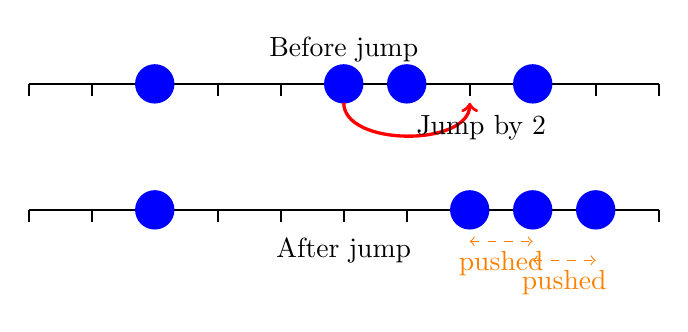
\begin{tikzpicture}[scale=0.8]
				% Before pushTASEP state
				\draw[thick] (0,2) -- (10,2);
				\foreach \x in {0,1,...,10}
								\draw[thick] (\x,2) -- (\x,1.8);

				% Particles before jump
				\node[circle, fill=blue, minimum size=0.5cm] at (2,2) {};
				\node[circle, fill=blue, minimum size=0.5cm] at (5,2) {};
				\node[circle, fill=blue, minimum size=0.5cm] at (6,2) {};
				\node[circle, fill=blue, minimum size=0.5cm] at (8,2) {};

				% Labels for before state
				\node[above] at (5,2.2) {Before jump};

				% Arrow indicating the jump
				\draw[->, very thick, red] (5,1.7) .. controls (5,1) and (7,1) .. (7,1.7);
				\node[right] at (6,1.3) {Jump by 2};

				% After pushTASEP state
				\draw[thick] (0,0) -- (10,0);
				\foreach \x in {0,1,...,10}
								\draw[thick] (\x,0) -- (\x,-0.2);

				% Particles after jump (particle at position 5 jumped and pushed the one at position 6)
				\node[circle, fill=blue, minimum size=0.5cm] at (2,0) {};
				\node[circle, fill=blue, minimum size=0.5cm] at (7,0) {};
				\node[circle, fill=blue, minimum size=0.5cm] at (8,0) {};
				\node[circle, fill=blue, minimum size=0.5cm] at (9,0) {};

				% Labels for after state
				\node[below] at (5,-0.3) {After jump};

				% Highlight pushed particles
				\draw[<->, dashed, orange] (7,-0.5) -- (8,-0.5) node[midway, below] {pushed};
				\draw[<->, dashed, orange] (8,-0.8) -- (9,-0.8) node[midway, below] {pushed};

\end{tikzpicture}
\caption{Illustration of a pushTASEP jump. The particle attempts to jump by 2. 
It pushes two particles in a cascade of pushes.}
\end{figure}
This connection completes the circle of relationships between random matrix theory, interacting particle systems, and last-passage percolation / random growth, demonstrating the deep unity of integrable probability models.

\appendix
\setcounter{section}{13}

\section{Problems (due 2025-04-29)}

\subsection{Non-Markovianity}

Show that the sequence of random variables defined in the exponential LPP model,
\[
L(1,n),L(2,n),\dots,L(t,n),
\]
is \textbf{not} a Markov chain.
By virtue of the equivalence with the spiked Wishart ensemble \eqref{eq:main-claim},
you may alternatively show that the sequence
of maximal eigenvalues
\[
\lambda_1(1),\lambda_1(2),\dots,\lambda_1(t)
\]
of successive
Wishart matrices $M(1),M(2),\dots,M(t)$ is \textbf{not} a Markov chain either.


\subsection{Schur polynomials --- equivalence of definitions}
\label{prob:Schur_polynomials_equivalence}

Show the equivalence of the two definitions of Schur polynomials \eqref{eq:Schur_polynomial} and \eqref{eq:Schur_polynomial_combinatorial}.

\medskip
\noindent
\textbf{Hint:}
Substitute $x_n=1$ and consider how both formulas
expand as linear combinations of Schur
polynomials
$s_\mu(x_1,\ldots,x_{n-1} )$
in $n-1$ variables.
This induction (together with the fact that
Schur polynomials are a linear basis in the ring
of symmetric polynomials in a given fixed number of variables)
will show that the two definitions are equivalent.

\subsection{Schur polynomials --- stability property}

Show the stability property of Schur polynomials \eqref{eq:stability_property_Schur}.


\subsection{Cauchy identity for Schur polynomials}
\label{prob:Cauchy_identity}

Let $a_1, \ldots, a_t$ and $b_1, \ldots, b_n$ be positive parameters satisfying $a_i b_j < 1$ for all pairs $(i,j)$. Prove the Cauchy identity for Schur polynomials:
\begin{equation*}
	\sum_{\mu: \mu_1 \geq \mu_2 \geq \cdots \geq \mu_n \geq 0} s_\mu(a_1,\ldots,a_t)s_\mu(b_1,\ldots,b_n) = \prod_{i=1}^t\prod_{j=1}^n \frac{1}{1-a_i b_j}.
\end{equation*}












\bibliographystyle{alpha}
\bibliography{bib}


\medskip

\textsc{L. Petrov, University of Virginia, Department of Mathematics, 141 Cabell Drive, Kerchof Hall, P.O. Box 400137, Charlottesville, VA 22904, USA}

E-mail: \texttt{lenia.petrov@gmail.com}


\end{document}
